% !TEX root = owasp-doc.tex
% \clearpage %%% Since this is the first section in the resources chapter, we don't clear the page

\textbf{OWASP Top 10 for Large Language Model Applications}
\begin{figure}[ht]
  \centering
  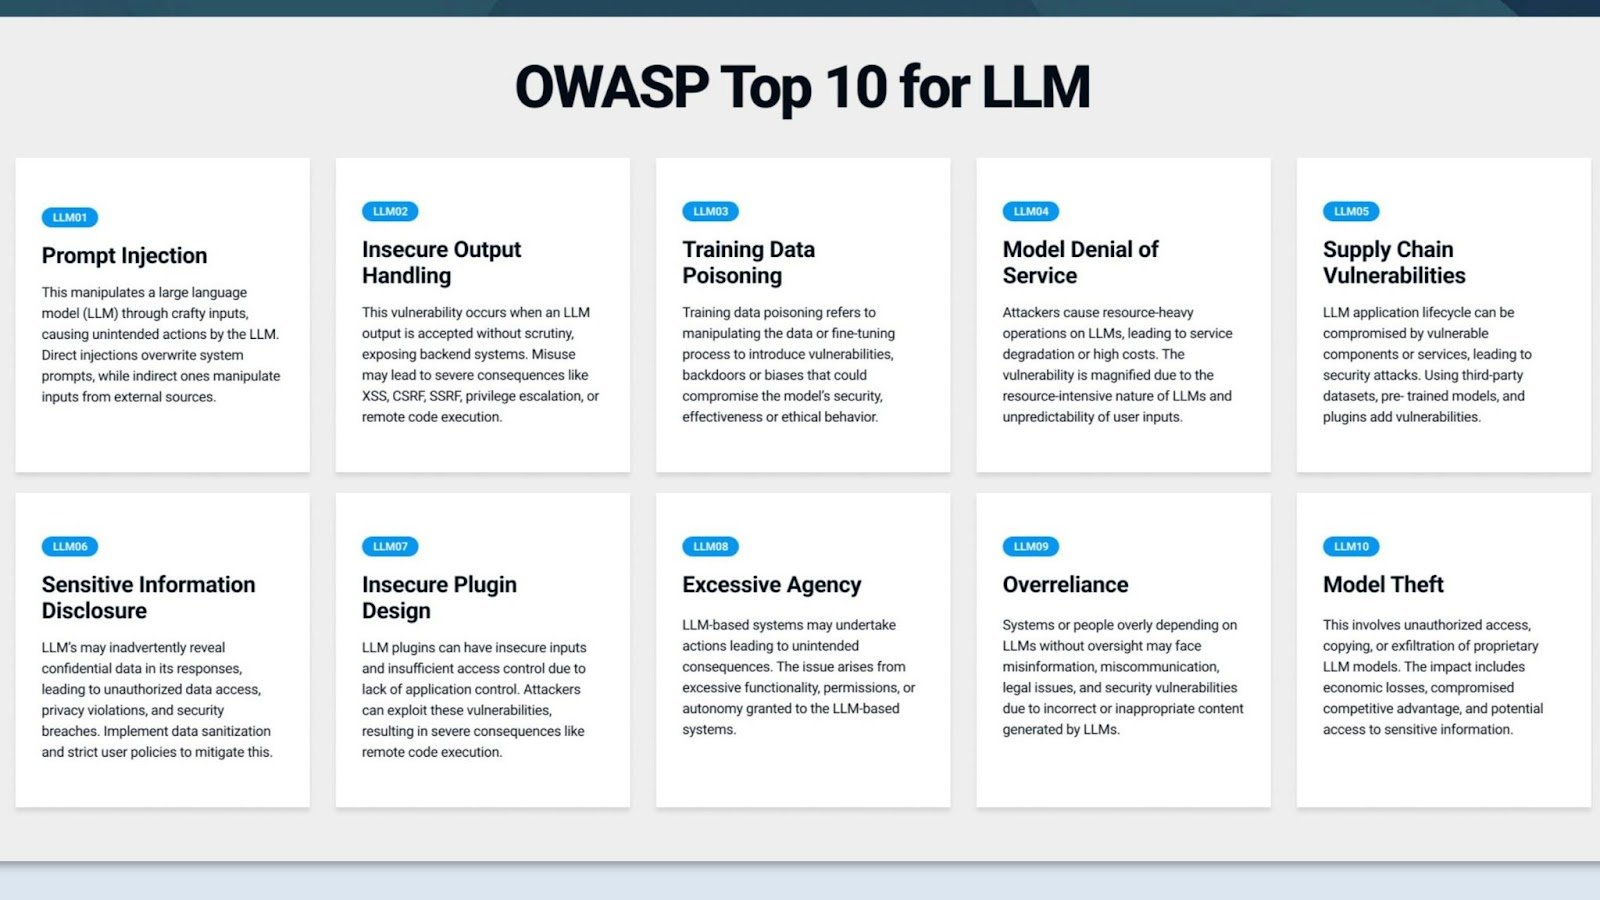
\includegraphics[width=0.8\textwidth]{owasp_top_10_llm_highlevel}
  \caption{Image of OWASP Top 10 for Large Language Model Applications}
  \label{fig:owasp-top-10-llm-highlevel}
\end{figure}

\clearpage
\textbf{OWASP Top 10 for Large Language Model Applications Visualized}
\begin{figure}[ht]
  \centering
  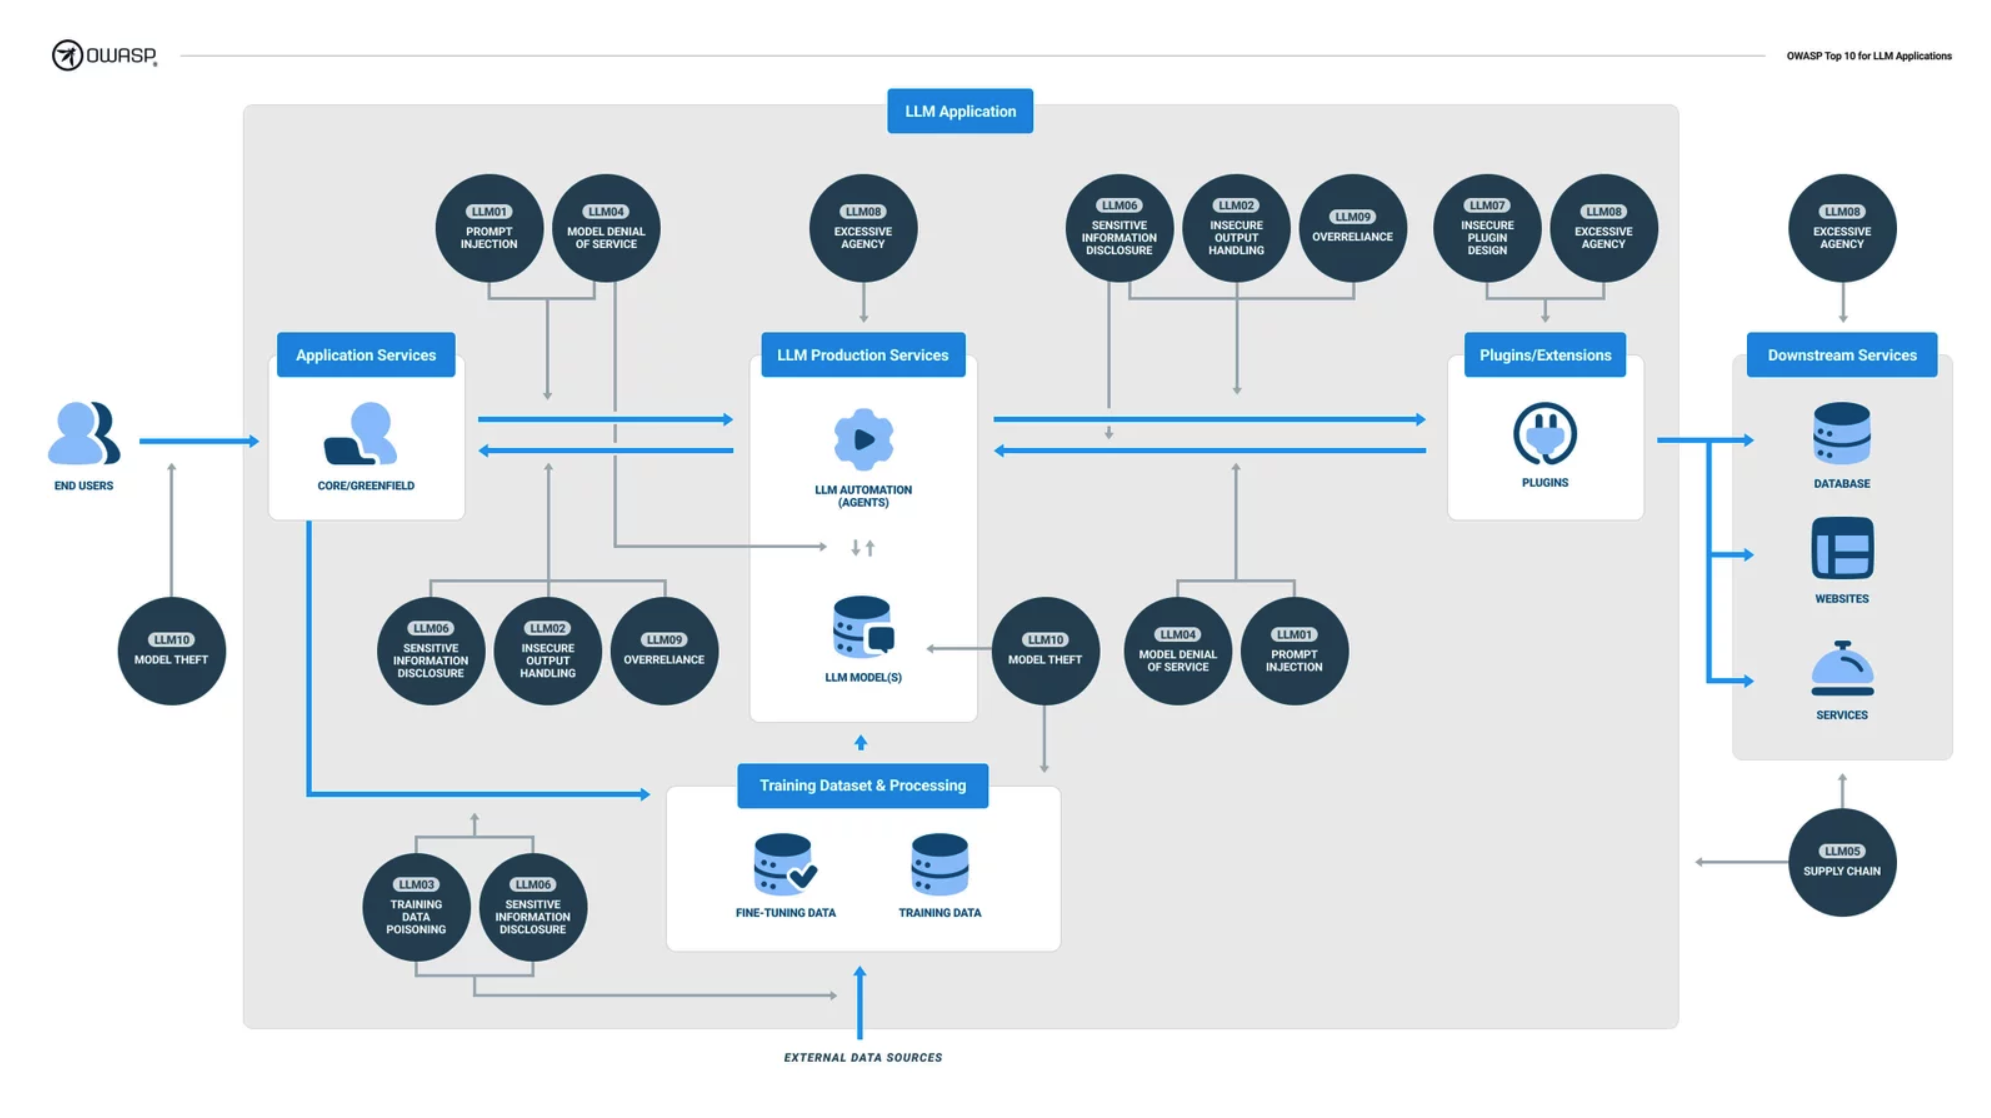
\includegraphics[width=0.8\textwidth]{owasp_top_10_llm_app_arch}
  \caption{Image of OWASP Top 10 for Large Language Model Applications Visualized}
  \label{fig:owasp-top-10-llm-visualized}
\end{figure}

\clearpage
\textbf{OWASP Resources}
Using LLM solutions expands an organization's attack surface and presents new
challenges, requiring special tactics and defenses. It also poses problems that
are similar to known issues, and there are already established cybersecurity
procedures and mitigations. Integrating LLM cybersecurity with an organization's
established cybersecurity controls, processes, and procedures allows an
organization to reduce its vulnerability to threats. How they integrate with
each other is available at the
\href{https://owasp.org/www-project-integration-standards/}{OWASP Integration Standards}.
%%% TABLE FORMATTING
\setlength\LTleft{0pt}
\setlength\LTright{0pt}
\begin{longtable}[c]{|p{0.25\textwidth}|p{0.25\textwidth}|p{0.35\textwidth}|}
  %%% Header and footer information
  \hline
  \rowcolor{owasplightpurple}
  \textbf{OWASP Resource} &
  \textbf{Description} &
  \textbf{Why It Is Recommended \& Where To Use It} \\
  \hline
  \endfirsthead
  \hline
  \rowcolor{owasplightpurple}
  \textbf{OWASP Resource} &
  \textbf{Description} &
  \textbf{Why It Is Recommended \& Where To Use It} \\
  \hline
  \endhead
  \endfoot
  %%% TABLE DATA GOES HERE
  \href{https://owasp.org/www-project-samm/}{OWASP SAMM}&
  Software Assurance Maturity Model &
  Provides an effective and measurable way to analyze and improve an
  organization's secure development lifecycle. SAMM supports the complete
  software lifecycle. It is interative and risk-driven, enabling organizations
  to identify and prioritize gaps in secure software development so resources
  for improving the process can be dedicated where efforts have the greatest
  improvement impact. \\
  \hline
  \href{https://owasp.org/www-project-ai-security-and-privacy-guide/}{OWASP AI Security and Privacy Guide} &
  OWASP Project with a goal of connecting worldwide for an exchange on AI
  security, fostering standards alignment, and driving collaboration. &
  The OWASP AI Security and Privacy Guide is a comprehensive list of the most
  important AI security and privacy considerations. It is meant to be a
  comprehensive resource for developers, security researchers, and security
  consultants to verify the security and privacy of AI systems. \\
  \hline
  \href{https://owasp.org/www-project-ai-security/}{OWASP AI Exchange} &
  OWASP AI Exchange is the intake method for the OWASP AI Security and Privacy Guide. &
  The AI Exchange is the primary intake method used by OWASP to drive the direction of
  the OWASP AI Security and Privacy Guide. \\
  \hline
  \href{https://mltop10.info/}{OWASP Machine Learning Security Top 10} &
  OWASP Machine Learning Security Top 10 security issues of machine learning systems. &
  The OWASP Machine Learning Security Top 10 is a community-driven effort to
  collect and present the most important security issues of machine learning
  systems in a format that is easy to understand by both a security expert and
  a data scientist. This project includes the ML Top 10 and is a live working
  document that provides clear and actionable insights on designing, creating,
  testing, and procuring secure and privacy-preserving AI systems. It is the
  best OWASP resource for AI global regulatory and privacy information.\\
  \hline
  \href{https://www.opencre.org/}{OpenCRE} &
  OpenCRE (Common Requirement Enumeration) is the interactive content-linking
  platform for uniting security standards and guidelines into one overview. &
  Use this site to search for standards. You can search by standard name or by
  control type.  \\
  \hline
  \href{https://owasp.org/www-community/Threat_Modeling}{OWASP Threat Modeling} &
  A structured, formal process for threat modeling of an application &
  Learn everything about Threat Modeling which is a structured representation
  of all the information that affects the security of an application. \\
  \hline
  \href{https://owasp.org/www-project-cyclonedx/}{OWASP CycloneDX} &
  OWASP CycloneDX is a full-stack Bill of Materials (BOM) standard that
  provides advanced supply chain capabilities for cyber risk reduction. &
  Modern software is assembled using third-party and open source components.
  They are glued together in complex and unique ways and integrated with
  original code to achieve the desired functionality. An SBOM provides an
  accurate inventory of all components which enables organizations to identify
  risk, allows for greater transparency, and enables rapid impact analysis.
  \href{https://www.nist.gov/itl/executive-order-14028-improving-nations-cybersecurity/software-security-supply-chains-software-1}{EO 14028}
  provided minimum requirements for SBOM for federal systems. \\
  \hline
  \href{https://scvs.owasp.org/}{OWASP Software Component Verification Standard (SCVS) } &
  A community-driven effort to establish a framework for identifying activities,
  controls, and best practices can help in identifying and reducing risk in a
  software supply chain. &
  Use SCVS to develop a common set of activities, controls, and best-practices
  that can reduce risk in a software supply chain and identify a baseline and
  path to mature software supply chain vigilance. \\
  \hline
  \href{https://owasp.org/www-project-api-security/}{OWASP API Security Project } &
  API Security focuses on strategies and solutions to understand and mitigate
  the unique vulnerabilities and security risks of Application Programming
  Interfaces (APIs) &
  APIs are a foundational element of connecting applications, and mitigating
  misconfigurations or vulnerabilities is mandatory to protect users and
  organizations. Use for security testing and red teaming the build and
  production environments. \\
  \hline
  \href{https://owasp.org/www-project-application-security-verification-standard/}{OWASP Application Security Verification Standard ASVS} &
  Application Security Verification Standard (ASVS) Project provides a basis
  for testing web application technical security controls and also provides
  developers with a list of requirements for secure development. &
  Cookbook for web application security requirements, security testing, and
  metrics. Use to establish security user stories and security use case release
  testing. \\
  \hline
  \href{https://owasp.org/www-project-threat-and-safeguard-matrix/}{OWASP Threat and Safeguard Matrix (TaSM)} &
  An action oriented view to safeguard and enable the business &
  This matrix allows a company to overlay its major threats with the NIST Cyber
  Security Framework Functions (Identify, Protect, Detect, Respond, \& Recover)
  to build a robust security plan. Use it as a dashboard to track and report on
  security across the organization. \\
  \hline
  \href{https://www.defectdojo.com/}{Defect Dojo} &
  An open source vulnerability management tool that streamlines the testing
  process by offering templating, report generation, metrics, and baseline
  self-service tools. &
  Use Defect Dojo to reduce the time for logging vulnerabilities with templates
  for vulnerabilities, imports for common vulnerability scanners, report
  generation, and metrics. \\
  \hline
  %%% TABLE DATA ENDS HERE
  \caption{OWASP Resources}
  \label{tab:owasp-resources}
\end{longtable}
